\includegraphics[height=1.25cm]{images/pictograms/FEM}
\includegraphics[height=1.25cm]{images/pictograms/3d}
\includegraphics[height=1.25cm]{images/pictograms/clean}

%%%%%%%%%%%%%%%%%%%%%%%%%%%%%%%%%%%%%%%%%%%%%%%%%%%%%%%%%%%%%%%%%%%%%%%%%%%%%%%%%%%%%%%%%

\lstinputlisting[language=bash,basicstyle=\small]{python_codes/fieldstone_10/keywords.key}

\begin{center}
\inpython
\injulia
\infortran
{\small Code: \url{https://github.com/cedrict/fieldstone/tree/master/python_codes/fieldstone_10}}
\end{center}

\par\noindent\rule{\textwidth}{0.4pt}
%%%%%%%%%%%%%%%%%%%%%%%%%%%%%%%%%%%%%%%%%%%%%%%%%%%%%%%%%%%%%%%%%%%%%%%%%%%%%%%%%%%%%%%%%

Last revision: August 30th, 2025.

\par\noindent\rule{\textwidth}{0.4pt}
%%%%%%%%%%%%%%%%%%%%%%%%%%%%%%%%%%%%%%%%%%%%%%%%%%%%%%%%%%%%%%%%%%%%%%%%%%%%%%%%%%%%%%%%%


%----------------------------------------------------------
\subsection*{Manufactured solution ({\tt experiment=5})}

It is described in Section~\ref{MMM-ss:mms3Dgen}.
The velocity and pressure fields are:
\begin{eqnarray}
u(x,y,z) &=& x(1-x)(1-2y)(1-2z)\\
v(x,y,z) &=& (1-2x) y(1-y) (1-2z) \\
w(x,y,z) &=& -2(1-2x)(1-2y)z(1-z) \\
p(x,y,z) &=& (2x-1)(2y-1)(2z-1)
\end{eqnarray}
This flow field has the built-in property that there is no flux through the 
boundaries, i.e. the normal component of the velocity field is zero on each face. 

\begin{center}
\includegraphics[width=5.6cm]{python_codes/fieldstone_10/results/exp5/press}
\includegraphics[width=5.6cm]{python_codes/fieldstone_10/results/exp5/vel}
\end{center}

\begin{center}
\includegraphics[width=5.6cm]{python_codes/fieldstone_10/results/exp5/vrms}
\includegraphics[width=5.6cm]{python_codes/fieldstone_10/results/exp5/conv}
\includegraphics[width=5.6cm]{python_codes/fieldstone_10/results/exp5/p_stats}
\end{center}
We recover the expected second order velocity error convergence 
and first order pressure error convergence. 
Surprisingly, we find that the results are not sensitive to the value of the penalty parameter $\lambda$.

This \stone is implemented in both python and julia, in order to look at
performance aspects. Both versions of the code are as close to each other 
as possible. The FE build and solve times are recorded and we find
that the build time grows linearly with the number of elements in the python 
case but not in the julia case. I suspected that the sparse storage of julia
(as opposed to a linked list converted to sparse matrix in python) makes it slow
so I ran the code without the assembly and indeed it is then linear with the 
number of elements.
I need to find a better way!!

\begin{center}
\includegraphics[width=8cm]{python_codes/fieldstone_10/results/exp5/julia/build.pdf}
\includegraphics[width=8cm]{python_codes/fieldstone_10/results/exp5/julia/solve.pdf}\\
{\captionfont Matrix building and system solve times for both python and julia codes.
Obtained with penalty=1e6. Each resolution is run 3 times.}
\end{center}


%----------------------------------------------------------
\subsection*{Aquarium ({\tt experiment=0})}

FS on all sides, $\rho=\eta=g_z=1$, $\lambda=10^6$

\begin{center}
\includegraphics[width=5.7cm]{python_codes/fieldstone_10/results/exp0/stats_uv}
\includegraphics[width=5.7cm]{python_codes/fieldstone_10/results/exp0/stats_w}
\includegraphics[width=5.7cm]{python_codes/fieldstone_10/results/exp0/stats_p}\\
{\captionfont Statistics of $u,v,w,p$.}
\end{center}

We expect a zero velocity field. This is the case (down to machine precision) for the $u$
and $v$ components, but since the penalty method yields a weakly compressible flow, 
the vertical component $w$ is larger but remains small.
The pressure is expected to be lithostatic and it should be -0.5 at the top and +0.5 at 
the bottom. Pressure statistics seem to converge towards these values. 





%------------------------------
\subsection*{Stokes sphere}

The domain is a unit cube. Free slip boundary conditions 
are imposed on all sides. The mesh counts 
nelx*nely*nelz=nel elements and 
nnx*nny*nnz=NV nodes.
The density and the viscosity are prescribed in the domain 
by means of two functions:
the density is set to $1+\delta \rho$ inside a sphere of radius 0.123456789 centered 
at (0.5,0.5,0.5) and 1 outside. The viscosity is 1000 inside the sphere
and 1 outside.  The gravity vector is set to $\vec{g}=(0,0,-1)$.
This is the benchmark presented in Section~\ref{MMM-ss:stokes_sphere_3D}.

The FE matrix size grows even faster now than in the previous 2D case so
choosing the right matrix storage is of paramount importance. 

Three experiments are carried out:
\begin{enumerate}
\item[Exp.~1:] the one described above.
Free slip or no slip boundary conditions.
We see that the pressure field is dominated by the lithostatic signal.
\item[Exp.~2:] same as experiment 1, but a reference density of 1 is substracted to all densities, so that 
the sphere density is 1 and the density of the surrounding fluid is now 0. In essence, we remove a
'background' density which does not participate in the flow generation, and thereby get rid of the 
lithostatic signal of the pressure.
Free slip or no slip boundary conditions.
\item[Exp.~3:] same as experiment 2, but the top boundary is now open (free surface)
\end{enumerate} 

\begin{center}
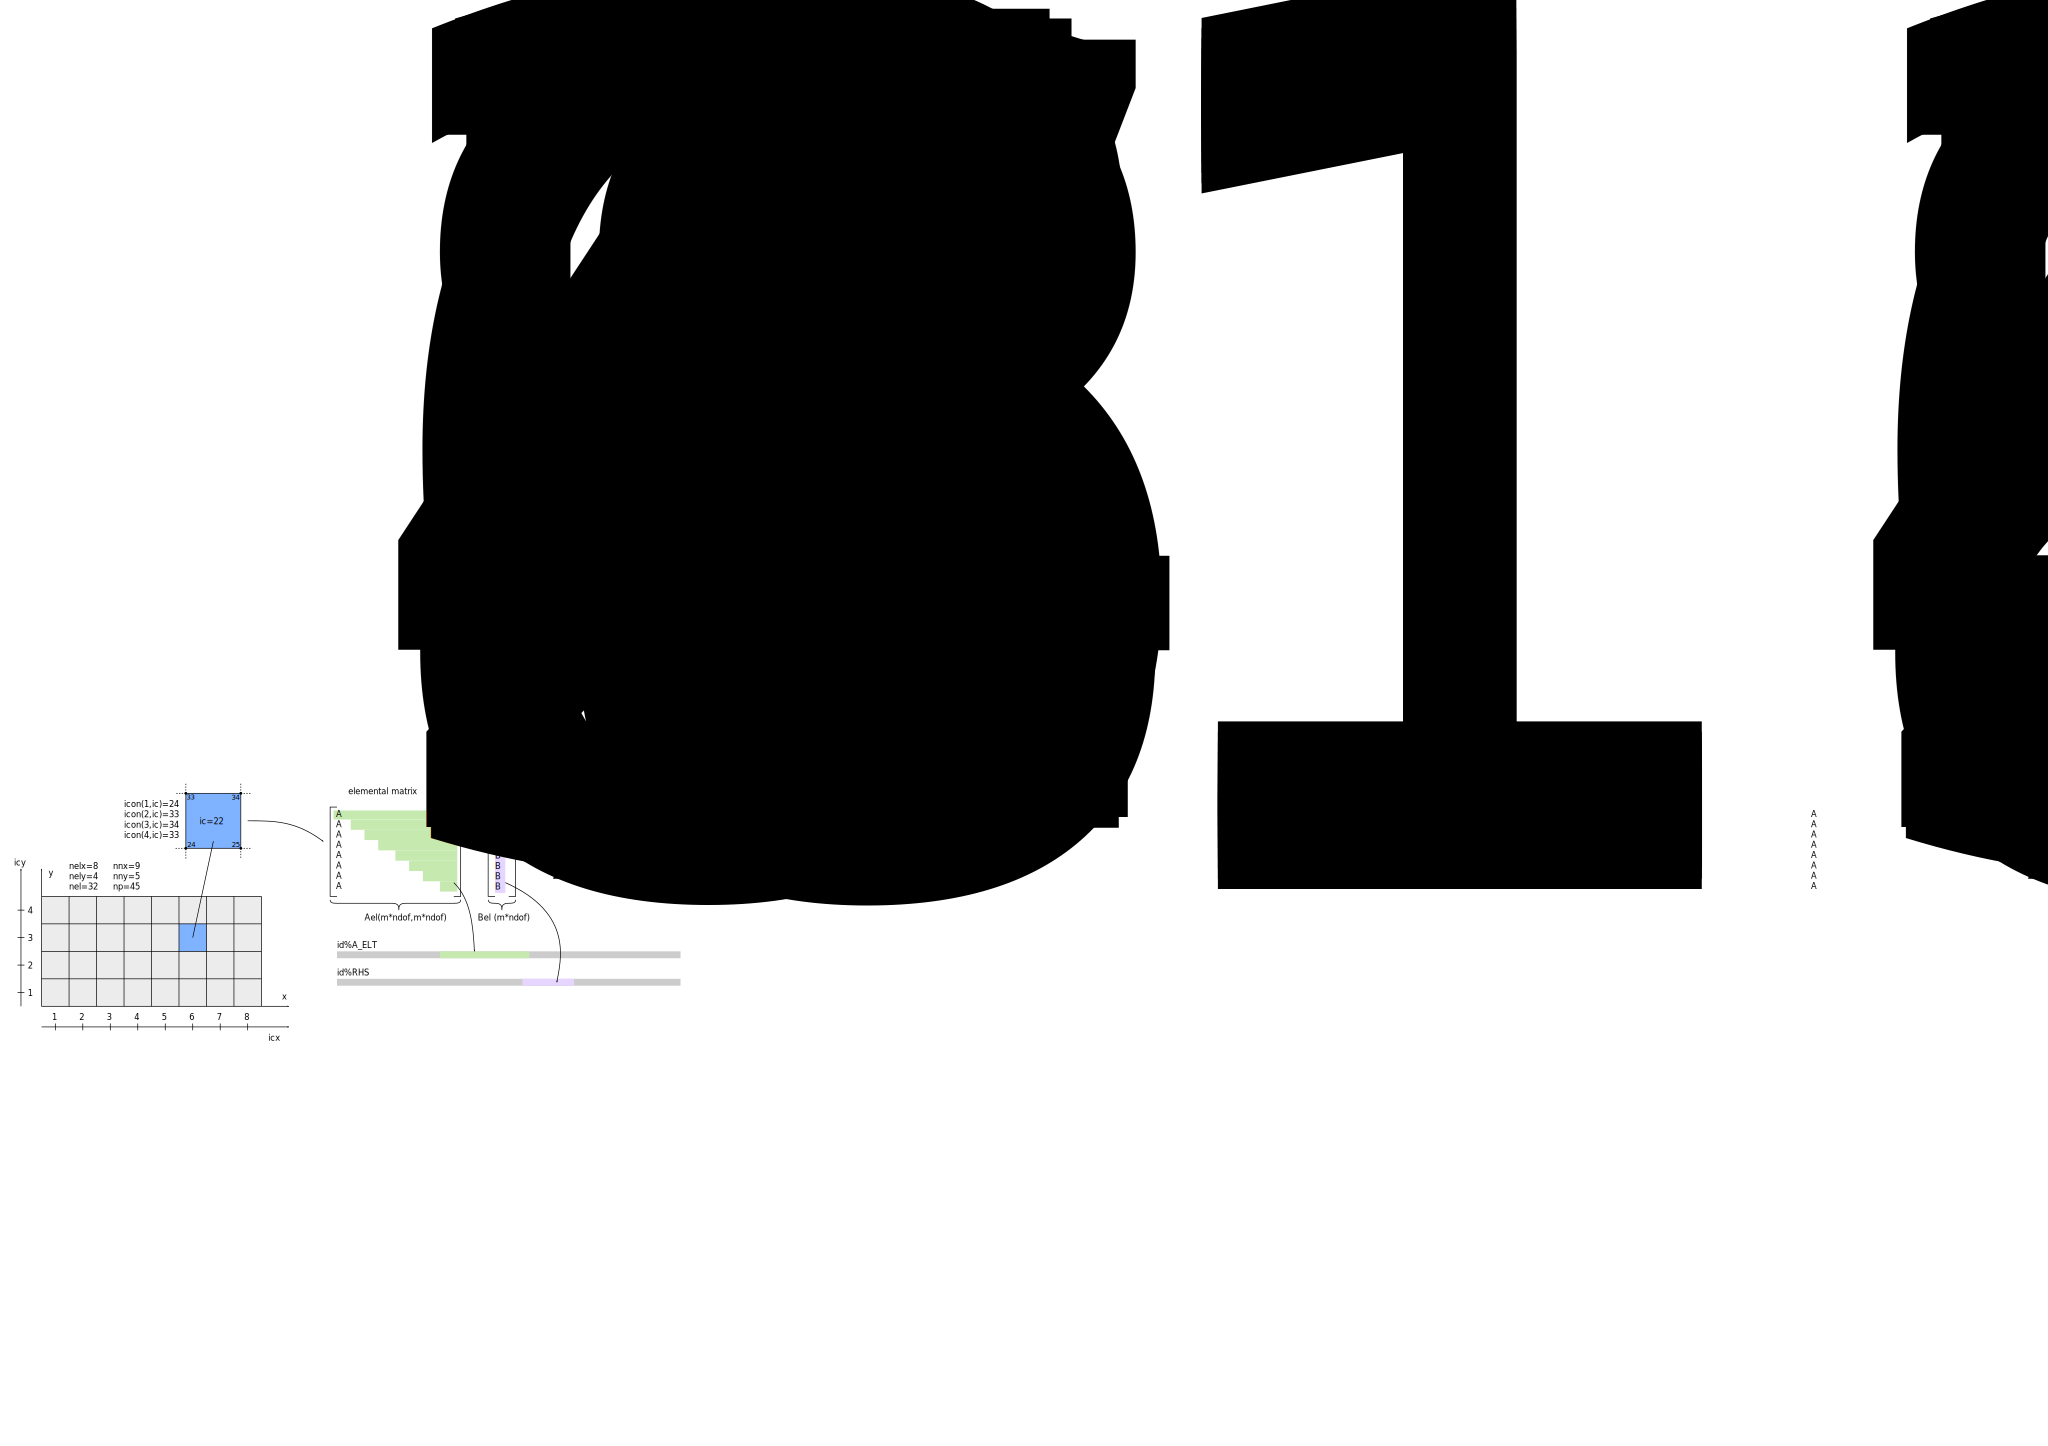
\includegraphics[width=5.7cm]{python_codes/fieldstone_10/results/exp1/grid}
\includegraphics[width=5.7cm]{python_codes/fieldstone_10/results/exp1/vel}
\includegraphics[width=5.7cm]{python_codes/fieldstone_10/results/exp1/press}\\
\includegraphics[width=5.7cm]{python_codes/fieldstone_10/results/exp1/visc}
\includegraphics[width=5.7cm]{python_codes/fieldstone_10/results/exp1/dens}\\
{\small Exp.~1: resolution $24\times 24\times 24$}
\end{center}

\begin{center}
\includegraphics[width=7cm]{python_codes/fieldstone_10/results/exp2/dens_2}
\includegraphics[width=7cm]{python_codes/fieldstone_10/results/exp2/press_2}\\
{\small Exp.~2: Density and pressure fields. Resolution 24x24x24}
\end{center}


\begin{center}
\includegraphics[width=7cm]{python_codes/fieldstone_10/results/exp3/press_3}
\includegraphics[width=7cm]{python_codes/fieldstone_10/results/exp3/vel_3}\\
{\small Exp.~3: pressure and velocity fields. Resolution 24x24x24}
\end{center}

\begin{center}
\includegraphics[width=5.6cm]{python_codes/fieldstone_10/results/exp1/pressure.pdf}
\includegraphics[width=5.6cm]{python_codes/fieldstone_10/results/exp2/pressure.pdf}
\includegraphics[width=5.6cm]{python_codes/fieldstone_10/results/exp3/pressure.pdf}\\
{\captionfont Elemental pressure for all elements as a function of their vertical 
(middle) coordinate for (from left to right) experiments 1, 2 and 3. }
\end{center}

Note that a similar fortran code is present in the folder. 

If the option 'quarter' is true, then the model takes advantage of the symmetries 
of the problem and runs it in a quarter of the original domain, so that 
the domain is then $0.5\times 0.5 \times 1$. Measurements/results are identical 
to the full cube ones, but at a much lower cost.

\begin{center}
\includegraphics[width=4cm]{python_codes/fieldstone_10/results/quarter_FS/press}
\includegraphics[width=4cm]{python_codes/fieldstone_10/results/quarter_FS/sr}
\includegraphics[width=4cm]{python_codes/fieldstone_10/results/quarter_FS/vel}
\includegraphics[width=4cm]{python_codes/fieldstone_10/results/quarter_FS/eta}\\
{\captionfont Resolution $32\times 32\times 64$ - FS}
\end{center}


\begin{center}
\includegraphics[width=7cm]{images/stokes_sphere3D/vrms_FS}
\includegraphics[width=7cm]{images/stokes_sphere3D/vrms_NS}\\
{\captionfont Left: FS; Right: NS. Results obtained with this stones and other ones, as well as ASPECT.
See Section~\ref{MMM-ss:stokes_sphere_3D} for all results.}
\end{center}

\newpage
%%%%%%%%%%%%%%%%%%%%%%%%%%%%%%%%%%%%%%%%%%%%%%%%%%%%%%%%
\section*{Trying $Q_2\times Q_0$+penalty... because why not}

Based on a discussion with A. Regorda I have coded a $Q_2\times Q_0$
(still with penalty) version of the \stone: {\tt stoneQ2Q0.py}.
The following results are obtained with {\tt script\_Q2Q0}.

I first naively used a 1 point integration (as for the 
$Q_1 \times P_0$ element) only for the 
penalty term, only to realise that the penalty term $\K_\lambda$ should be 
under-integrated, but not necessarily using a single point. 

This sparked the study on the influence of the quadrature rule 
of the penalty term on the accuracy of results.

I also implemented the consistent pressure recovery described 
in Section~\ref{MMM-ss:cpr}.
This results in a nodal pressure field (which I call $q$) which is 
solution of 
\[
{\bm M} \cdot \vec{Q} = \vec{f}
\]
where ${\bm M}$ is the $Q_2$ mass matrix that 
is integrated with the same quadrature as the viscous block $\K_\eta$
but the rhs $\vec{f}$ is integrated with the same quadrature as 
the penalty block $\K_\lambda$.
In the end I also keep the pressure $p$ computed in the middle of the element
using $p= \lambda \vec\nabla\cdot \vec\upnu$.

Finally to save time I have used the fact that the Jacobian of the 
coordinate change for cuboids is a diagonal matrix containing terms $h_x/2$,
$h_y/2$, $h_z/2$ on the diagonal. This means that this can be computed once
and for all for all elements. 

%----------------------------------------------------------
\subsection*{Aquarium ({\tt experiment=0})}

Fress slip on all sides, $\rho=\eta=g_z=1$, $\lambda=10^6$

\begin{center}
\includegraphics[width=5.7cm]{python_codes/fieldstone_10/resultsQ2/exp0/errv}
\includegraphics[width=5.7cm]{python_codes/fieldstone_10/resultsQ2/exp0/errp}
\includegraphics[width=5.7cm]{python_codes/fieldstone_10/resultsQ2/exp0/errq}\\
\includegraphics[width=8cm]{python_codes/fieldstone_10/resultsQ2/exp0/p_stats}
\end{center}

We expect a zero velocity field. This is the case (down to machine precision) 
for the $u$ and $v$ components, but since the penalty method yields a 
weakly compressible flow, the vertical component $w$ is much larger 
then $u$ and $v$.
The pressure is expected to be lithostatic and it should be -0.5 at the top 
and +0.5 at the bottom. Pressure statistics to converge towards these values. 

\begin{center}
\includegraphics[width=5cm]{python_codes/fieldstone_10/resultsQ2/exp0/press}
\includegraphics[width=5cm]{python_codes/fieldstone_10/resultsQ2/exp0/w}\\
{\captionfont $w$ and $p$ for resolution $20\times 20 \times 20$.}
\end{center}

Note that at resolution 20x20x20 build time is 10min, and solve time is 48 min!
Given this 'performance' this will limit a lot the tests we can carry out...

%----------------------------------------------------------
\subsection*{Manufactured solution ({\tt experiment=5})}

See Section~\ref{MMM-ss:mms3Dgen} for the analytical expressions 
of the velocity, pressure and body force vector.

\begin{center}
\includegraphics[width=5.7cm]{python_codes/fieldstone_10/resultsQ2/exp5/errv}
\includegraphics[width=5.7cm]{python_codes/fieldstone_10/resultsQ2/exp5/errp}
\includegraphics[width=5.7cm]{python_codes/fieldstone_10/resultsQ2/exp5/errq}\\
\includegraphics[width=8cm]{python_codes/fieldstone_10/resultsQ2/exp5/vrms}
\includegraphics[width=8cm]{python_codes/fieldstone_10/resultsQ2/exp5/p_stats}
\end{center}

Since the analytical solution of this experiment is quadratic then the 
velocity basis functions can exactly represent the solution inside each
element and the accuracy of the velocity solution depends on the penalty parameter and
not on resolution.
We clearly see that using only one integration point for the penalty term results
in lesser accurate velocities.
Interestingly we obtain a superconvergence (third order) of the $q$ error 
for a 2x2x2 quadrature and only a linear convergence for the $q$ error
for a 3x3x3 quadrature.
The pressure $q$ obtained with only 1 quad point yields results that are so off
that they do not show on the plots.
Finally we note that we obtain pressures that often exceed the analytical 
bounds for min and max pressure except for $q$ with 2x2x2 quadrature.
This seems to indicate that a 2x2x2 quadrature is preferable.
We keep investigating in the next section with a more suitable manufactured
solution benchmark.

\begin{center}
\includegraphics[width=5.7cm]{python_codes/fieldstone_10/resultsQ2/exp5/vel}
\includegraphics[width=5.7cm]{python_codes/fieldstone_10/resultsQ2/exp5/p}
\includegraphics[width=5.7cm]{python_codes/fieldstone_10/resultsQ2/exp5/q}\\
{\captionfont $||\vec\upnu||$, $p$ and $q$ for resolution $20\times 20 \times 20$.}
\end{center}

%----------------------------------------------------------
\subsection*{Manufactured solution ({\tt experiment=6})}

After the observations made about the previous experiment we then turn to 
another 3D manufactured solution as described in Section~\ref{MMM-ss:mms3Dgen}.

\begin{eqnarray}
f(x) &=& x^2(1-x)^2 \\
g(y) &=& y^2(1-y)^2 \\
h(z) &=& z^2(1-z)^2 \\
u(x,y,z) &=& fg'h' \\
v(x,y,z) &=& f'gh'  \\
w(x,y,z) &=& -2f'g'h \\
p(x,y,z) &=& -f'g'h'
\end{eqnarray}


\begin{center}
\includegraphics[width=5.7cm]{python_codes/fieldstone_10/resultsQ2/exp6/errv}
\includegraphics[width=5.7cm]{python_codes/fieldstone_10/resultsQ2/exp6/errp}
\includegraphics[width=5.7cm]{python_codes/fieldstone_10/resultsQ2/exp6/errq}\\
\includegraphics[width=5.7cm]{python_codes/fieldstone_10/resultsQ2/exp6/vrms}
\includegraphics[width=5.7cm]{python_codes/fieldstone_10/resultsQ2/exp6/p_stats}
\includegraphics[width=5.7cm]{python_codes/fieldstone_10/resultsQ2/exp6/q_stats}
\end{center}

We find that:
\begin{itemize}
\item The velocity error exhibits cubic convergence {\it only} 
for $2\times 2\times 2$ quadrature and is the smallest.
\item the convergence of the $p$ pressure is puzzling
\item the convergence of the $q$ pressure is second order (!) for 
$2\times 2\times 2$ quadrature and is also the smallest.   
\end{itemize}

The conclusion is clear: {\color{violet}the penalty term $\K_\lambda$ 
must be integrated with $2\times 2\times 2$ quadrature}.

TODO: determine analytical min max of pressure

